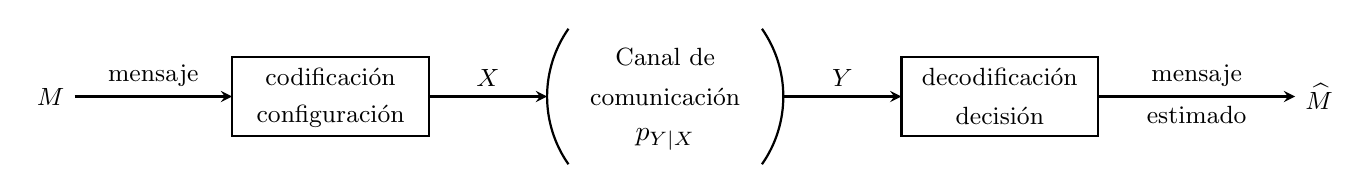
\begin{tikzpicture}
\shorthandoff{>}
%
% Mensaje
\draw[>=stealth,->,thick] (0,0) node[left]{\small $M$} --(2,0);
\draw (1,0) node[above]{\small mensaje};
%
% codificacion
\draw[thick] (2,-.5) rectangle (4.5,.5);
\draw (3.25,.25) node{\small codificaci\'on};
\draw (3.25,-.25) node{\small configuraci\'on};
%
% entrada del canal
\draw[>=stealth,->,thick] (4.5,0)--(6,0);
\draw (5.25,0) node[above]{\small $X$};
%
% Canal de com
\pgfmathsetmacro{\t}{35};
\pgfmathsetmacro{\r}{1.5};
\draw[thick] ({6+\r*(1+cos(180-\t))},{\r*sin(\t)}) arc (180-\t:180+\t:\r);
\draw[thick] ({6+\r*(1+cos(\t))},{-\r*sin(\t)}) arc (-\t:\t:\r);
\draw ({6+\r},.5) node{\small Canal de};
\draw ({6+\r},0) node{\small comunicaci\'on};
\draw ({6+\r},-.55) node{$p_{Y|X}$};
%
% salida
\draw[>=stealth,->,thick] ({6+2*\r},0)--({7.5+2*\r},0);
\draw ({6.75+2*\r},0) node[above]{\small $Y$};
%
% decodificacion/decision
\draw[thick] ({7.5+2*\r},-.5) rectangle ({10+2*\r},.5);
\draw ({8.75+2*\r},.25) node{\small decodificaci\'on};
\draw ({8.75+2*\r},-.25) node{\small decisi\'on};
%
% Mensaje estimado
\draw[>=stealth,->,thick] ({10+2*\r},0)--({12.5+2*\r},0) node[right]{\small $\widehat{M}$};
\draw ({11.25+2*\r},0) node[above]{\small mensaje};
\draw ({11.25+2*\r},0) node[below]{\small estimado};
\end{tikzpicture}
